\chapter{AI as Your Daily Business Assistant}

\epigraph{The best way to predict the future is to invent it. But sometimes, the best way to invent it is to let AI handle the tedious parts.}{Adapted from Alan Kay}

The most immediate return on AI investment is not a moonshot initiative. It is replacing thirty minutes of tedious work every single day. Summarizing email threads. Restructuring meeting notes. Drafting routine responses. Preparing for client calls. The low-hanging fruit.

This chapter focuses on using AI as a daily business assistant---the patterns, prompts, and habits that compound into significant productivity gains without requiring IT involvement or formal project approval.

\section{The Low-Hanging Fruit}

Not all work deserves your full attention. Some tasks are repetitive, low-stakes, text-heavy, and time-consuming. These are ideal candidates for AI assistance.

\subsection{Four Criteria for AI-Ready Tasks}

A task becomes a good AI candidate when it meets most of these criteria:

\begin{table}[htbp]
\centering
\begin{tabularx}{\textwidth}{lX}
\toprule
\textbf{Criterion} & \textbf{What This Means} \\
\midrule
Repetitive & You do it multiple times per week \\
Low-stakes & Errors are easy to catch and fix \\
Text-heavy & Input and output are primarily text \\
Time-consuming & Takes 15+ minutes of focused work \\
\bottomrule
\end{tabularx}
\caption{Criteria for identifying AI-ready tasks}
\end{table}

Tasks that fit these criteria include summarizing long email threads before responding, converting meeting notes into action items, drafting routine status updates, extracting key points from reports, translating customer communications, and creating first drafts of standard documents.

Tasks that do not fit include strategic decisions requiring judgment, legal documents with compliance requirements, anything containing confidential data (more on this in Section~\ref{sec:boundaries}), and novel problems with no clear pattern. The common thread: if the task requires deep expertise, carries significant risk, or involves sensitive information, keep it human.

\begin{roicalc}[Time Saved Compounds]
If AI saves you 30 minutes per day on routine tasks:
\begin{itemize}
    \item \textbf{Per week:} 2.5 hours
    \item \textbf{Per month:} 10 hours (more than one full workday)
    \item \textbf{Per year:} 120 hours (three full work weeks)
\end{itemize}

That is three weeks you can redirect to high-value work---strategic planning, relationship building, creative problem solving---or simply leaving work at a reasonable hour.
\end{roicalc}

\begin{figure}[htbp]
\centering
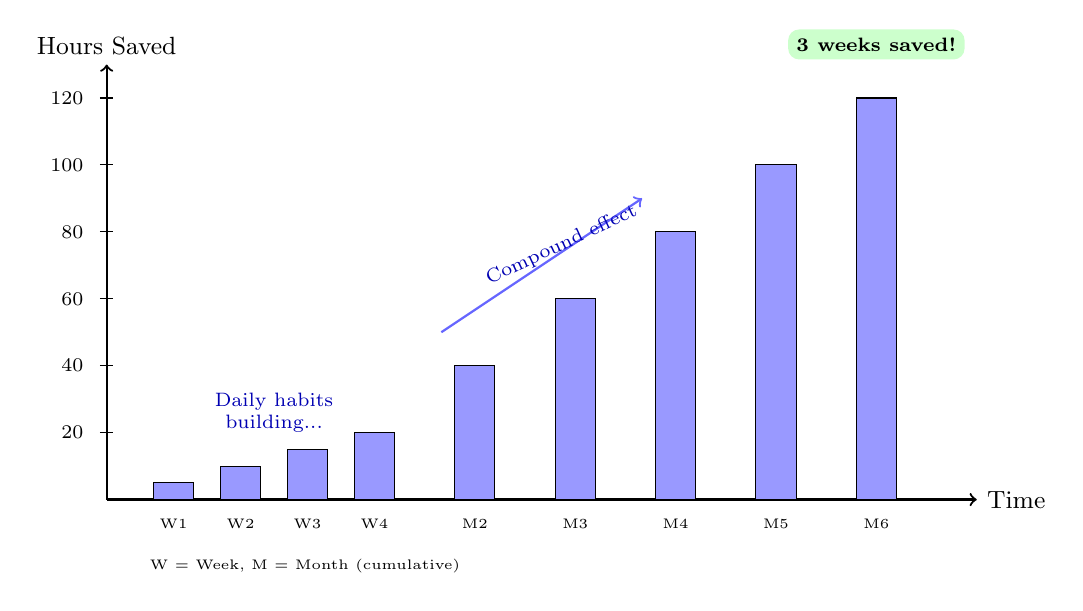
\begin{tikzpicture}[scale=0.85]
    % Y-axis
    \draw[thick, ->] (0,0) -- (0,6.5) node[above, font=\small] {Hours Saved};

    % X-axis
    \draw[thick, ->] (0,0) -- (13,0) node[right, font=\small] {Time};

    % Y-axis labels
    \foreach \y/\label in {1/20, 2/40, 3/60, 4/80, 5/100, 6/120} {
        \draw (-0.1,\y) -- (0.1,\y);
        \node[left, font=\scriptsize] at (-0.2,\y) {\label};
    }

    % Bars with cumulative time saved
    \foreach \x/\h/\label in {1/0.25/W1, 2/0.5/W2, 3/0.75/W3, 4/1/W4, 5.5/2/M2, 7/3/M3, 8.5/4/M4, 10/5/M5, 11.5/6/M6} {
        \fill[blue!40] (\x-0.3,0) rectangle (\x+0.3,\h);
        \draw[black] (\x-0.3,0) rectangle (\x+0.3,\h);
        \node[below, font=\tiny] at (\x,-0.15) {\label};
    }

    % Annotations
    \node[font=\scriptsize, text=blue!70!black, align=center] at (2.5, 1.3) {Daily habits\\building...};

    \draw[thick, ->, blue!60] (5, 2.5) -- (8, 4.5);
    \node[font=\scriptsize, text=blue!70!black, rotate=25] at (6.8, 3.8) {Compound effect};

    % Highlight final result
    \node[fill=green!20, rounded corners, font=\scriptsize, inner sep=3pt] at (11.5, 6.8) {\textbf{3 weeks saved!}};

    % Legend
    \node[font=\tiny, anchor=west] at (0.5, -1) {W = Week, M = Month (cumulative)};

\end{tikzpicture}
\caption{The Compound Effect of Daily AI Time Savings: 30 minutes per day becomes 120 hours (three work weeks) per year}
\label{fig:time-savings-compound}
\end{figure}

\section{Effective Prompting Fundamentals}

The quality of AI output depends directly on the quality of your prompt. A vague prompt produces vague results. A structured prompt produces useful results.

\subsection{The Five-Part Prompt Structure}

Effective prompts follow a consistent structure. Not every prompt needs all five parts, but knowing the structure helps you construct better requests.

\begin{framework}[Five-Part Prompt Template]
\begin{enumerate}
    \item \textbf{Role:} Who should the AI act as? (e.g., ``You are an executive assistant...'')
    \item \textbf{Task:} What specific action do you want? (e.g., ``Summarize this email thread...'')
    \item \textbf{Context:} What background information matters? (e.g., ``This is about a delayed project...'')
    \item \textbf{Constraints:} What limitations apply? (e.g., ``Keep it under 5 bullet points...'')
    \item \textbf{Output format:} What should the result look like? (e.g., ``Use bullet points with action items...'')
\end{enumerate}
\end{framework}

\subsection{Poor vs. Better Prompts}

Let's see this structure in action with real examples.

\begin{promptexample}[Poor Prompt]
Summarize this email.
\end{promptexample}

\textbf{Problem:} Too vague. How long should the summary be? What aspects matter? What will you do with this summary?

\begin{promptexample}[Better Prompt]
You are my executive assistant helping me catch up after being out of office.

Summarize this email thread in 3-5 bullet points focusing on:
- Key decisions that were made
- Any action items directed at me
- Urgent matters requiring response

Format: Start with "URGENT" if anything needs immediate attention, then bullet points.
\end{promptexample}

\textbf{Why this works:} The AI knows the context (catching up), the focus (decisions and actions), the constraints (3-5 points), and the format (bullets with urgent flag).

\begin{promptexample}[Poor Prompt]
Make this email better.
\end{promptexample}

\textbf{Problem:} ``Better'' is subjective. Shorter? More formal? More friendly? The AI will guess.

\begin{promptexample}[Better Prompt]
I'm writing to a long-time client who we disappointed with a project delay.

Rewrite this email to be:
- Genuinely apologetic without making excuses
- Clear about our plan to fix it
- Professional but warm (we have a 5-year relationship)

Keep it under 200 words. Maintain my core message but improve the tone.
\end{promptexample}

\textbf{Why this works:} Clear context (disappointed client, long relationship), specific tone requirements (apologetic, professional, warm), concrete constraint (200 words).

\begin{tip}[Start with Structure, Not Polish]
Your first attempts at structured prompts will feel awkward and verbose. That is fine. Focus on clarity, not elegance. Once you see results improve, you will naturally develop your own style.
\end{tip}

\section{Turning Raw Text into Clarity}

One of AI's most immediately useful capabilities is transforming text: summarizing long documents, extracting key information, and restructuring content for different purposes.

\subsection{Summarization That Actually Helps}

Generic summaries are useless. ``This document discusses project status.'' Great. You knew that already.

Useful summaries extract what matters for your specific purpose.

\begin{promptexample}[Generic Summarization]
Summarize this 10-page project status report.
\end{promptexample}

\begin{promptexample}[Targeted Summarization]
I'm a department head reviewing this project status report before our weekly executive meeting.

Extract and summarize:
1. Red flags or blockers requiring escalation (list first)
2. Key milestones achieved this period
3. Budget variance (if mentioned)
4. Changes to timeline

Format: Use a numbered list. Flag any item needing executive decision with [DECISION NEEDED].
\end{promptexample}

The second prompt produces actionable output because it specifies your role, your purpose, and what decisions you need to make.

\subsection{Extraction: Finding Needles in Haystacks}

AI excels at pulling specific information from large documents.

\begin{promptexample}[Extraction Example]
I need to prepare for a contract negotiation.

From this 40-page agreement draft, extract:
- All dates and deadlines
- Payment terms and amounts
- Penalty clauses
- Any "shall" vs. "may" language (indicates obligations)
- Sections marked for legal review

Present as a table with: Section, Topic, Key Terms, and Urgency Level.
\end{promptexample}

This turns forty pages into a one-page reference sheet you can actually use in a meeting.

\subsection{Restructuring for Different Audiences}

The same information needs different structure for different audiences.

\begin{realexample}[One Report, Three Audiences]
A project manager had a detailed technical status report. She needed to present the same information to:
\begin{itemize}
    \item Her technical team (full detail)
    \item Her VP (executive summary)
    \item The client (focusing on business value)
\end{itemize}

Instead of manually creating three versions, she used AI:

\textbf{For the VP:}
\begin{quote}
\texttt{Rewrite this technical report for a VP who needs to understand business impact, not technical details. Focus on: timeline, budget, risks, and what decisions she needs to make. Maximum 1 page.}
\end{quote}

\textbf{For the client:}
\begin{quote}
\texttt{Rewrite this focusing on business outcomes and value delivered. Remove internal technical details. Emphasize how this meets their original requirements. Use client-friendly language, not jargon.}
\end{quote}

\textbf{Result:} Three tailored documents in 15 minutes instead of 2+ hours of manual rewriting.
\end{realexample}

\begin{keyinsight}
AI does not care about your writing style, your title, or your domain. It transforms text based on the structure you specify. The more specific your output requirements, the more useful the result.
\end{keyinsight}

\section{Working Across Languages and Cultures}

Translation is an obvious AI use case. But effective translation goes beyond word-for-word conversion.

\subsection{Translation With Context}

Modern AI translators are dramatically better than earlier tools because they understand context. But you still need to provide it.

\begin{promptexample}[Basic Translation]
Translate this email from English to Spanish.
\end{promptexample}

\begin{promptexample}[Translation With Context]
Translate this customer service email from English to Spanish (Latin American Spanish, not Castilian).

Context: This is responding to a complaint about a delayed shipment. The customer is a long-term client. We want to sound apologetic and professional, but not overly formal.

After translating, note any phrases where cultural context might affect the tone.
\end{promptexample}

The second version accounts for regional differences (Latin American vs. Castilian Spanish), relationship context, and asks the AI to flag cultural considerations you might miss.

\subsection{Cultural Adaptation}

Sometimes you need more than translation---you need cultural adaptation.

\begin{casestudy}{Marketing Copy Across Cultures}
A software company prepared a marketing campaign for their project management tool. The US version emphasized:
\begin{itemize}
    \item Individual productivity gains
    \item Competitive advantage
    \item Fast-paced innovation
\end{itemize}

Before launching in Japan and Germany, they used AI to adapt the messaging:

\textbf{Prompt:}
\begin{quote}
\texttt{This marketing copy is for US audiences. I need versions for: (1) Japanese business culture, and (2) German business culture.}

\texttt{For each version:}
\texttt{- Translate to the appropriate language}
\texttt{- Adapt messaging to emphasize values important in that culture}
\texttt{- Flag any claims that might sound boastful or inappropriate}
\texttt{- Suggest adjustments to imagery/examples that would resonate better}
\end{quote}

\textbf{Result:} The AI-suggested adaptations emphasized team harmony and process improvement for Japan, and reliability and engineering excellence for Germany. The marketing team refined these suggestions with local partners, but the AI draft saved weeks of back-and-forth and caught cultural nuances they would have missed.
\end{casestudy}

\begin{tip}[Verify With Native Speakers]
AI-generated translations and adaptations are excellent starting points, but always have a native speaker review anything customer-facing or business-critical. AI provides speed, not perfection.
\end{tip}

\section{Setting Boundaries and Guardrails}
\label{sec:boundaries}

AI tools are powerful, but they are not private. Everything you input might be used to train future models or stored by the provider. Treat AI chat interfaces like public forums.

\subsection{What NOT to Put Into AI Tools}

\begin{warning}[Never Share These With AI]
\begin{itemize}
    \item Customer data (names, emails, account details)
    \item Employee personal information
    \item Unreleased financial results
    \item Proprietary algorithms or source code
    \item Strategic plans not yet public
    \item Legal documents under attorney-client privilege
    \item Health information (HIPAA protected)
    \item Anything covered by NDA
    \item Passwords, API keys, credentials
    \item Competitive intelligence
\end{itemize}
\end{warning}

\textbf{The rule:} If you would not post it on your public website, do not put it in an AI chat.

\subsection{Safe Alternatives for Sensitive Work}

You can still use AI for sensitive domains---you just need to anonymize or use private deployments.

\begin{framework}[Working Safely With Sensitive Information]
\textbf{Option 1: Anonymize}
\begin{itemize}
    \item Replace names with ``Customer A,'' ``Employee 1''
    \item Replace specific numbers with realistic ranges
    \item Remove identifying details while preserving structure
\end{itemize}

\textbf{Example:}
\begin{quote}
Original: ``We need to address Sarah Chen's complaint about the Q4 pricing for XYZ Corp's enterprise contract.''

Anonymized: ``We need to address a long-term customer's complaint about quarterly pricing on an enterprise contract.''
\end{quote}

\textbf{Option 2: Private Deployment}
\begin{itemize}
    \item Enterprise AI tools (Microsoft 365 Copilot, Claude Enterprise, etc.)
    \item Data is not used for training
    \item Contractual privacy guarantees
    \item Your IT team controls access and retention
\end{itemize}

\textbf{Option 3: Avoid Sensitive Content Entirely}
\begin{itemize}
    \item Use AI for structure and approach, not specific content
    \item Ask ``How should I structure a response to a customer complaint?'' not ``Draft this response to XYZ Corp''
    \item Get templates and patterns, fill in specifics yourself
\end{itemize}
\end{framework}

\subsection{Organizational Policies}

If you manage a team or department, establish clear guidelines before problems occur.

\begin{checklist}[AI Usage Policy Checklist]
\begin{itemize}
    \item[$\square$] What AI tools are approved for use?
    \item[$\square$] What types of information can/cannot be shared?
    \item[$\square$] Who approves exceptions for sensitive use cases?
    \item[$\square$] How should team members anonymize data?
    \item[$\square$] Are there audit/logging requirements?
    \item[$\square$] What happens if someone violates policy?
    \item[$\square$] How often will we review and update this policy?
\end{itemize}
\end{checklist}

\begin{keyinsight}
The goal is not to prevent AI use---it is to prevent careless disclosure. Clear policies let your team use AI confidently without creating risk.
\end{keyinsight}

\section{Simple Daily Habits That Compound}

Occasional AI use provides occasional benefits. Daily habits compound into significant productivity gains.

\subsection{Morning Routine: Start Your Day With AI}

\textbf{Habit 1: Email Triage (5 minutes)}

Before diving into your inbox, get AI to pre-process it.

\begin{promptexample}[Morning Email Triage]
I have 47 unread emails from the past 24 hours. I'll paste the subject lines and senders below.

Categorize these into:
1. URGENT - Needs response today
2. IMPORTANT - Needs response this week
3. FYI - Read when you have time
4. IGNORE - Newsletters, automated notifications

For URGENT items, note what decision or action is likely needed.
\end{promptexample}

\textbf{Time saved:} 15-20 minutes of reading through low-priority emails to find the urgent ones.

\textbf{Habit 2: Meeting Prep (5 minutes)}

\begin{promptexample}[Meeting Preparation]
I have a meeting in 30 minutes about [topic]. Here are my notes/agenda/previous discussions.

Prepare me by:
1. Summarizing the key issues
2. Listing likely questions I'll be asked
3. Identifying any decisions I need to make
4. Suggesting 2-3 good questions I should ask

Keep it concise---I need to read this in under 3 minutes.
\end{promptexample}

\textbf{Time saved:} 15 minutes of manually reviewing documents and preparing talking points.

\subsection{Meeting Routine: Capture and Process}

\textbf{Habit 3: Notes to Action Items (Immediately After Meetings)}

Do not let meeting notes sit in a document forever.

\begin{promptexample}[Meeting Notes Processing]
Here are my notes from a project planning meeting.

Extract:
1. Decisions made (with brief rationale)
2. Action items (who, what, when)
3. Open questions that need follow-up
4. Any risks or concerns mentioned

Format as a structured email I can send to the team within 10 minutes.
\end{promptexample}

\textbf{Time saved:} 20-30 minutes of manual note cleanup and action item extraction.

\textbf{Habit 4: Draft Responses to Common Requests}

\begin{promptexample}[Standard Response Drafting]
I frequently get asked [common question]. Here's the information I usually provide: [paste your standard response].

Draft a professional, friendly response I can customize and send in 2 minutes. Include placeholders for [specific details I'll fill in].
\end{promptexample}

Save these as templates. Over time, build a library of AI-refined responses for recurring situations.

\subsection{Weekly Habits: Reflection and Planning}

\textbf{Habit 5: Weekly Status Updates (Friday Afternoon)}

\begin{promptexample}[Status Report Generation]
I'm writing my weekly status update. Here are my notes on what I worked on this week: [paste notes].

Create a status update with:
- 3-5 key accomplishments
- Challenges encountered
- Plans for next week
- Any help needed from management

Format for my manager who prefers brief, results-focused updates.
\end{promptexample}

\textbf{Habit 6: Planning Next Week (Friday or Monday)}

\begin{promptexample}[Weekly Planning Assistant]
Here's my calendar for next week and my current priorities: [paste info].

Help me plan by:
1. Identifying scheduling conflicts
2. Suggesting which tasks I should batch together
3. Flagging any meetings where I'm under-prepared
4. Recommending which low-priority items I should defer

Give me a realistic plan assuming 6 productive hours per day (accounting for interruptions).
\end{promptexample}

\begin{roicalc}[Daily Habits: The Compound Effect]
Conservative estimate using AI habits daily:

\begin{tabular}{lr}
\toprule
\textbf{Habit} & \textbf{Time Saved (minutes/day)} \\
\midrule
Email triage & 15 \\
Meeting prep & 10 \\
Meeting notes processing & 20 \\
Status updates/planning (weekly) & 5 (daily average) \\
\midrule
\textbf{Total} & \textbf{50 minutes/day} \\
\bottomrule
\end{tabular}

\textbf{Per year:} 200+ hours saved (five full work weeks)

This is not theoretical. These are real, measurable time savings from replacing tedious work with AI-assisted work.
\end{roicalc}

\subsection{Building Your Own AI Habit Stack}

The habits above are starting points. The most effective habits are personal---tailored to your specific role and pain points.

\begin{framework}[Designing Your AI Habit]
\begin{enumerate}
    \item \textbf{Identify a pain point:} What repetitive task drains your time?
    \item \textbf{Test the prompt:} Spend 10 minutes crafting a good prompt for it
    \item \textbf{Refine based on results:} Adjust until output is consistently useful
    \item \textbf{Make it routine:} Do it at the same time/trigger every day for 2 weeks
    \item \textbf{Measure the impact:} Did it actually save time? Keep, modify, or drop
\end{enumerate}
\end{framework}

Common opportunities for AI habits include creating first drafts of recurring documents, preparing for specific types of meetings, reviewing and summarizing reports, drafting routine communications, extracting data from unstructured text, and researching topics before decisions. Look for tasks that consume time disproportionate to their strategic value---those are your best candidates.

\begin{tip}[Start Smaller Than You Think]
Do not try to build six new AI habits simultaneously. Pick one. Do it daily for two weeks. Once it is automatic, add another. Sustainable change happens through small, consistent improvements, not through ambitious overhauls that fade in a week.
\end{tip}

\section{Summary}

AI as a daily assistant is not about replacing your judgment or creativity. It is about reclaiming time from tedious, repetitive work and redirecting it toward high-value activities.

The low-hanging fruit is everywhere: summarization, extraction, restructuring, translation, drafting. These tasks are ideal for AI because they are repetitive, text-heavy, and low-stakes.

Effective prompting follows a structure: role, task, context, constraints, and output format. Vague prompts produce vague results. Specific prompts produce useful results.

But with power comes responsibility. Never share sensitive information with public AI tools. Anonymize when necessary, use private deployments for sensitive work, or avoid specific content entirely.

The real gains come from daily habits that compound. Email triage, meeting prep, notes processing, status updates---small time savings that add up to weeks per year. Start with one habit. Make it routine. Then add another.

Your goal is not to use AI for everything. Your goal is to identify the repetitive tasks that drain your time and systematically replace them with AI-assisted workflows. The time you save is time you can spend on work that actually requires your expertise, judgment, and creativity.

\begin{exercise}
Identify three repetitive tasks you do weekly that meet the criteria: repetitive, low-stakes, text-heavy, time-consuming. For each task, write a structured prompt (role, task, context, constraints, format) and test it with an AI tool. Document the time saved.
\end{exercise}

\begin{exercise}
Create a personal ``never share with AI'' list based on your role and industry. Share it with your team or manager to ensure alignment with organizational policies.
\end{exercise}

\begin{exercise}
Implement one AI habit for two weeks. Track the time saved per use. At the end of two weeks, evaluate: Is this habit worth keeping? How could you refine the prompt to make it even more useful?
\end{exercise}
